\chapter{1988 - CYB i USA!}

\author{Av Morten Moen \& Ole Christian Lingjærde}

\section{Planlegging og reise}

Det var tidlig på vinteren i 1988 at tanken om en tur til USA ble født. Det semesteret satt Morten som styreleder i CYB, og slik han husker det var det på et improvisert styremøte i Sky-baren på toppen av det tidligere SAS-hotellet at idéen ble formet. CYB hadde vært der før, men denne gangen skulle det gjøres større og bedre.

Ole Christian samarbeidet med Morten om programmet for oppholdet, og med Aina Hegdalsaunet om å arrangere reisen. Etter hvert ble reiseruta som følger:

\begin{itemize}
	\item Fly Oslo $\to$ New York og New York $\to$ Boston
	\item Besøk på Apollo Computer, Thinking Machines, MITs AI-Lab og Media-Lab, og Boston Computer Museum
	\item Fly Boston $\to$ San Francisco 
	\item Besøk på Sun Microsystems og Amdahl
	\item Biletappe San Francisco $\to$ Los Angeles
	\item Fly Los Angeles $\to$ Orlando
	\item Fly Orlando $\to$ New York $\to$ Oslo
\end{itemize}

Et hovedfokus i planleggingen var Amdahl Computers. Hos de andre firmaene CYB besøkte var det kun kontakt via mail, men hos Amdahl ble Ole Christian og Morten invitert på et møte på kontoret i Oslo, så det var tydelig at de syntes det var stas med noen som viste interesse i dem. Dette firmaet, som sluttet å eksistere i 1997, ble startet av Gene Amdahl og produserte store mainframemaskiner. Hans foreldre hadde utvandret fra Norge og Sverige, så de syntes det var gøy å få besøk av norske studenter.

Det snakkes om at å fly har blitt veldig billig nå, men det var også mulig å få rimelige billetter den gangen! Selve reiseplanleggingen ble som sagt tatt hånd om av Ole Christian og Aina, og de gjorde en fantastisk jobb. Å fly med Tjæreborg tur/retur New York kostet totalt 4870 kroner. Dette er kanskje ikke er så \textit{vanvittig} billig, men de hadde et opplegg med CIS Tours som kom godt til nytte. Fordi det ble booket tur/retur med Tjæreborg fikk CYB alle de andre flightene innad i USA for \$75, ergo New York $\to$ Boston $\to$ San Francisco og Los Angeles $\to$ Orlando $\to$ New York, som må kunne kalles relativt rimelig. 

Så mandag 12. september fløy 17 studenter fra det som da var charterterminalen på Gardermoen, med et flyselskap som het Tower Air. De startet opp i 1983, kunne tilby rimelige flybilletter, og kan sies å ha hatt et nokså uformelt crew. Flyene deres var gamle fly fra andre selskaper, og på beltene på flyet 12. september sto det klart og tydelig PanAm.

Da alle hadde funnet setene sine begynte en av cybberne å fikle med knappene i taket for å prøve å få på leselyset. Da dette ikke gikk tilkalte han en flyvert, som i dette tilfellet var en to meter høy og solid mann med en ganske kraftig stemme; et prakteksemplar av arten. Den før omtalte cybberen forklarte at knappen til leselyset ikke fungerte, hvorpå denne noe storvokste mannen bøyde seg over ham, og lyktes selvsagt umiddelbart med å få på lyset. Flyverten så deretter ned på cybberen, som var nokså liten i forhold, og sa: One more question, and you don't eat. Riktignok med et glimt i øyet, men det kom ingen flere spørsmål i løpet av turen.

Det ble bare én overnatting i New York, på Royce Hotel rett ved LaGuardia-flyplassen. Så godt som alle møtte til frokost i restauranten på hotellet, som ikke var inkludert, og derfor ble betalt av hver enkelt. Etterhvert som folk ble ferdige betalte de sin del og forlot restauranten, men da de siste hadde betalt det som sto på sin regning og skulle til å gå smalt det. Rasende kelnere som forlangte å få korrekt tips, og det ble tydelig at tips IKKE er valgfritt i USA, som var en viktig lekse å lære.

Dagen etterpå gikk turen videre til Boston, et av hovedstoppene på turen. Her sjekket cybberne inn på Best Western Homestead Inn, litt utenfor sentrum. Oppholdet der varte i fem dager mens CYB besøkte flere interessante bedrifter, blant dem Apollo Computer. 

\begin{figure}
	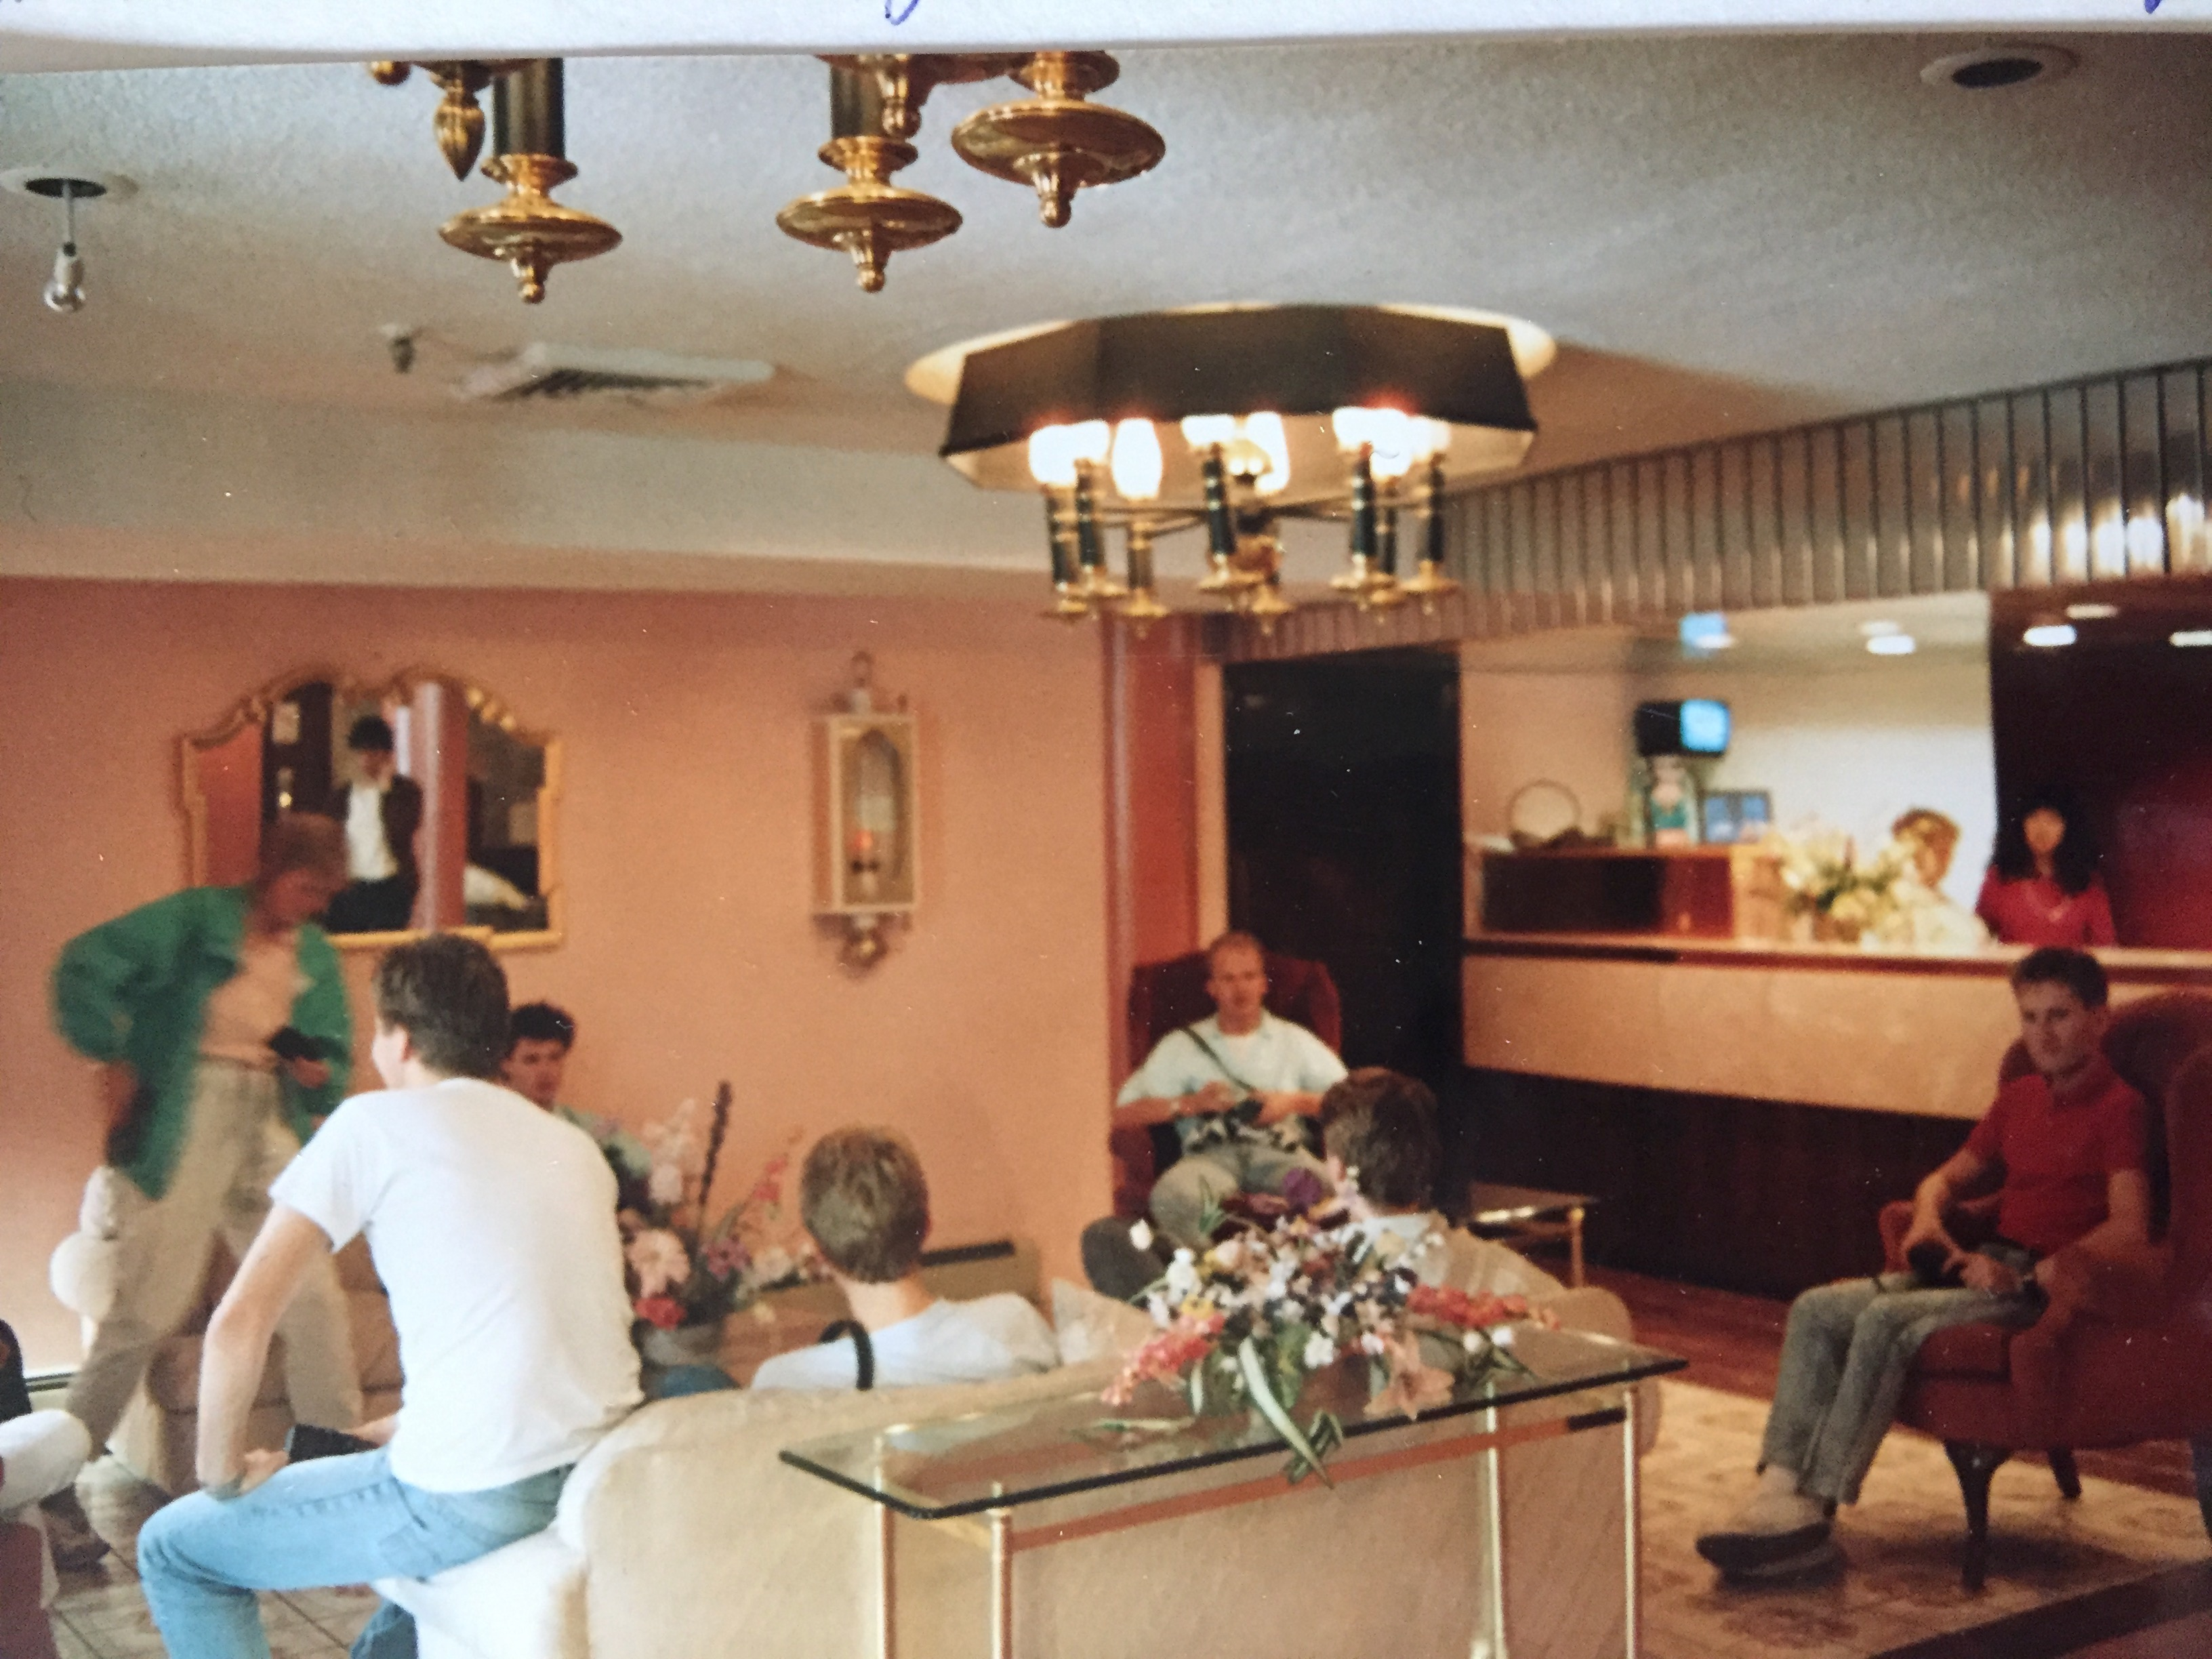
\includegraphics[width=\linewidth]{images/tur-til-usa-1988/IMG_3846.jpg}
	\caption{Fra resepsjonen på hotellet i Boston. Fra venstre: Anne Schiestad (i farta), ukjent (med ryggen til), Ole Christian Lingjærde, ukjent (med ryggen til), Geir Amdal, ukjent.}
\end{figure}

\section{Besøk hos Apollo Computer}

Natten før Apollo-besøket ble Morten vekket av lyden av sikkerhetslenken på døren på hotellrommet: noen hadde låst opp døren og forsøkt å komme inn, og blitt stoppet av lenken. Morten antok at det kanskje var noen ansatte som prøvde å ta seg inn på feil rom eller noe slikt. Senere, da cybberne samlet seg for å spise frokost ble det klart hva som hadde skjedd: I løpet av natten og morgenen hadde det vært et innbruddsraid på hotellet.

Gruppen var stort sett fordelt på tremannsrom på hotellet. På ett av rommene, da innbruddene tok sted, var det én som hadde gått ut, én som sto på badet, og én som fortsatt lå og sov i sengen. Han som var på badet hørte døren gå opp og noen komme inn, men antok det var romkameraten som hadde gått ut som kom inn igjen, og bestemte seg derfor for å ikke sjekke det, og den sovende våknet ikke. Etter en kort stund gikk personen ut igjen, og hadde fått med seg en klokke fra rommet deres.

Apollo ventet oss tidlig på formiddagen, men på grunn av tyveriet måtte de som bodde på det omtalte rommet bli igjen for å anmelde saken, og av en eller annen grunn følte flere andre at de burde være igjen litt og hjelpe dem. Dette resulterte i at den første gruppen som kom frem til Apollo var relativt liten. 

\begin{wrapfigure}{l}{6.5cm}
	\centering
	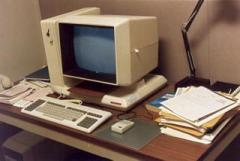
\includegraphics[width=0.45\textwidth]{images/tur-til-usa-1988/apollo_workstation.jpg}
	\caption{En Apollo arbeidsstasjon fra slutten av 80-tallet}
\end{wrapfigure}

På 80-tallet var Apollo Computer et av de største navnene innen grafiske arbeidsstasjoner. I tiårets første halvdel var Apollo verdens største produsent av nettverks-arbeidsstasjoner, og i 1986 ble firmaet også størst på ''engineering workstations''. De hadde da en dobbelt så stor markedsandel som Sun, som lå på andreplass. Apollo begynte derimot sin nedgang i slutten av 1987, og var altså på vei nedover da CYB var der. De ble kjøpt opp av HP året etterpå, og mye av teknologien deres gikk inn i HPs 9000-serie av maskiner.

Der hadde de likevel slått på stortromma for besøket og linet opp flere ledere, inkludert Europa-sjefen for Apollo, i et møterom for å fortelle om firmaet. De ble møtt med de 4-5 cybberne i den første puljen, og fikk en slags forklaring om at det hadde vært innbrudd på ett av rommene og at alle de andre måtte være igjen på hotellet fordi en hadde fått klokken sin stjålet. Stemningen var pinlig en stund, men da resten av gruppen kom kunne programmet endelig starte.

Besøket hos Apollo var forøvrig starten på en trend som fortsatte gjennom alle stedene CYB besøkte; foreningen ble tatt veldig seriøst, og ble veldig godt mottatt. Jevnt over ble cybberne møtt av høytstående mennesker som hadde stelt i stand store og innholdsrike opplegg. 

\begin{figure}[h!]
	\centering
	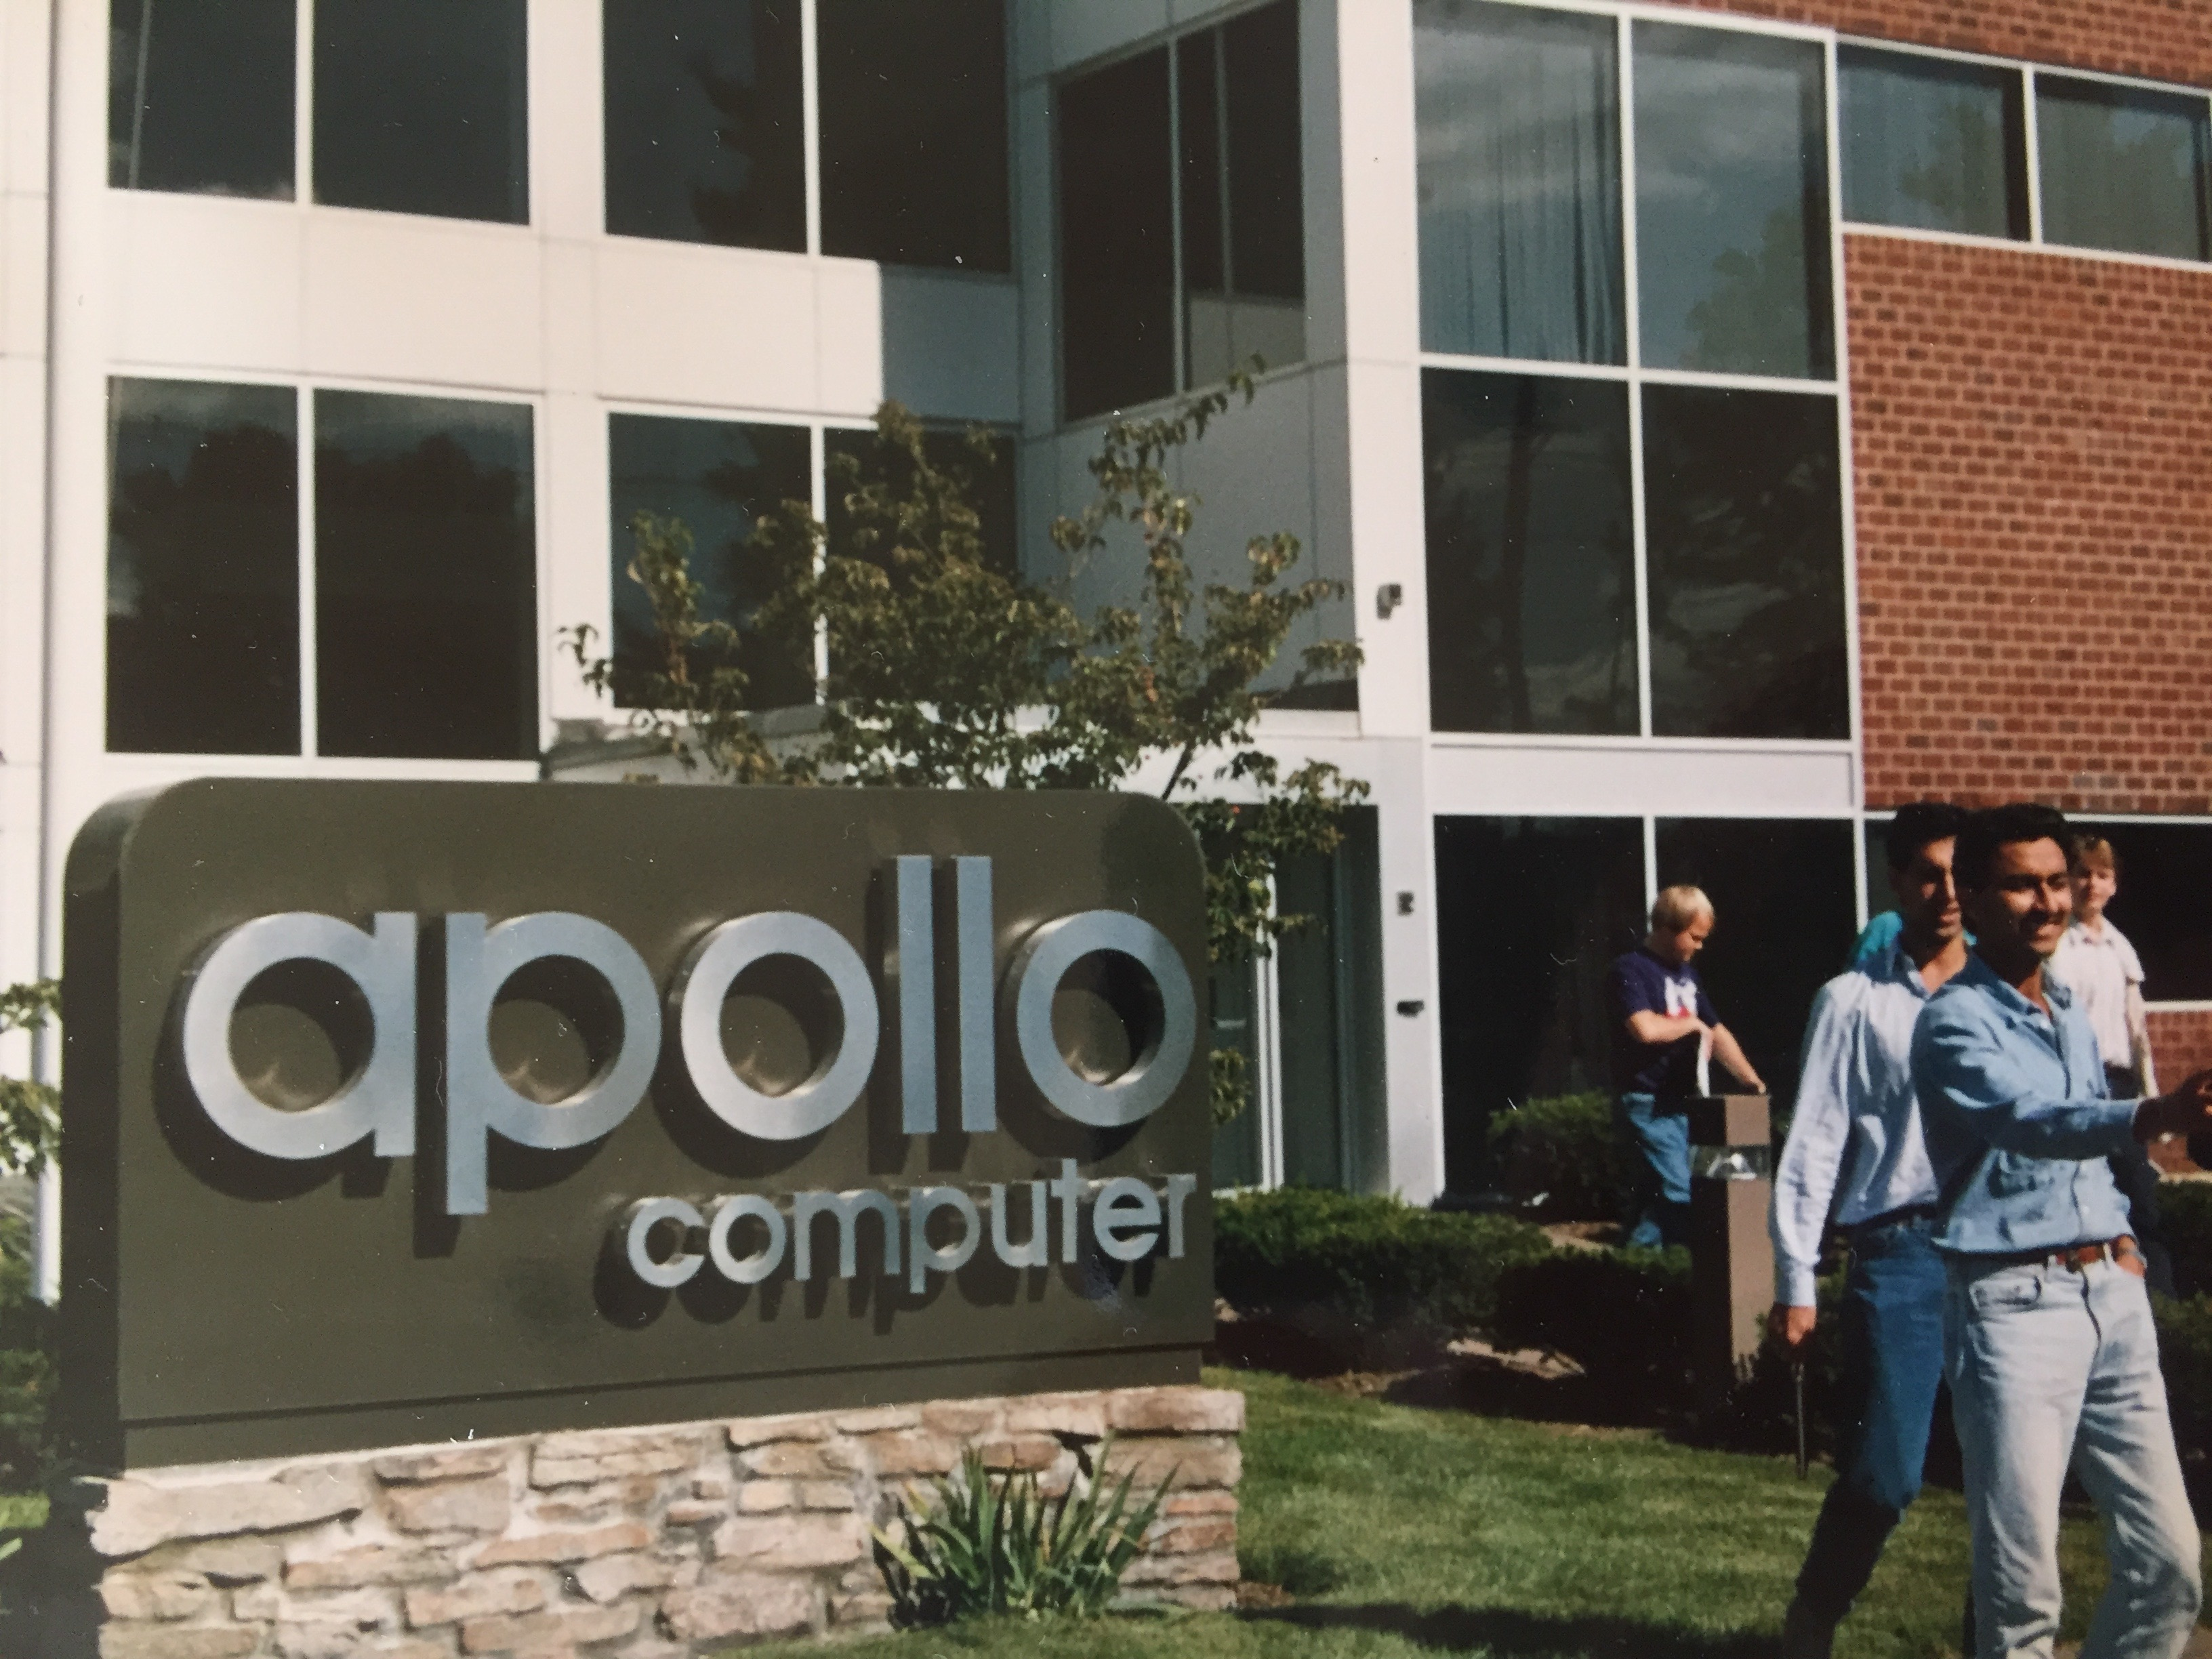
\includegraphics[width=0.7\textwidth]{images/tur-til-usa-1988/IMG_3790.jpg}
	\caption{Noen av oss på vei ut fra Apollo Computers.}
\end{figure}

\section{Besøk hos Thinking Machines Corporation}

Ett av besøkene alle gledet seg til var hos Thinking Machines Corporation i Boston, som var noe av en kuriositet. Thinking Machines ble startet i 1983 av Danny Hillis og var firmaet bak en supercomputer som het Connection Machine, basert på arbeid Hillis gjorde under doktorgraden sin hos MIT. Der hadde han blitt veiledet av blant annet Marvin Minsky, en av grunnleggerne av AI, og Claude Shannon, en av grunnleggerne av informasjonsteori. 

\begin{figure}
	\centering
	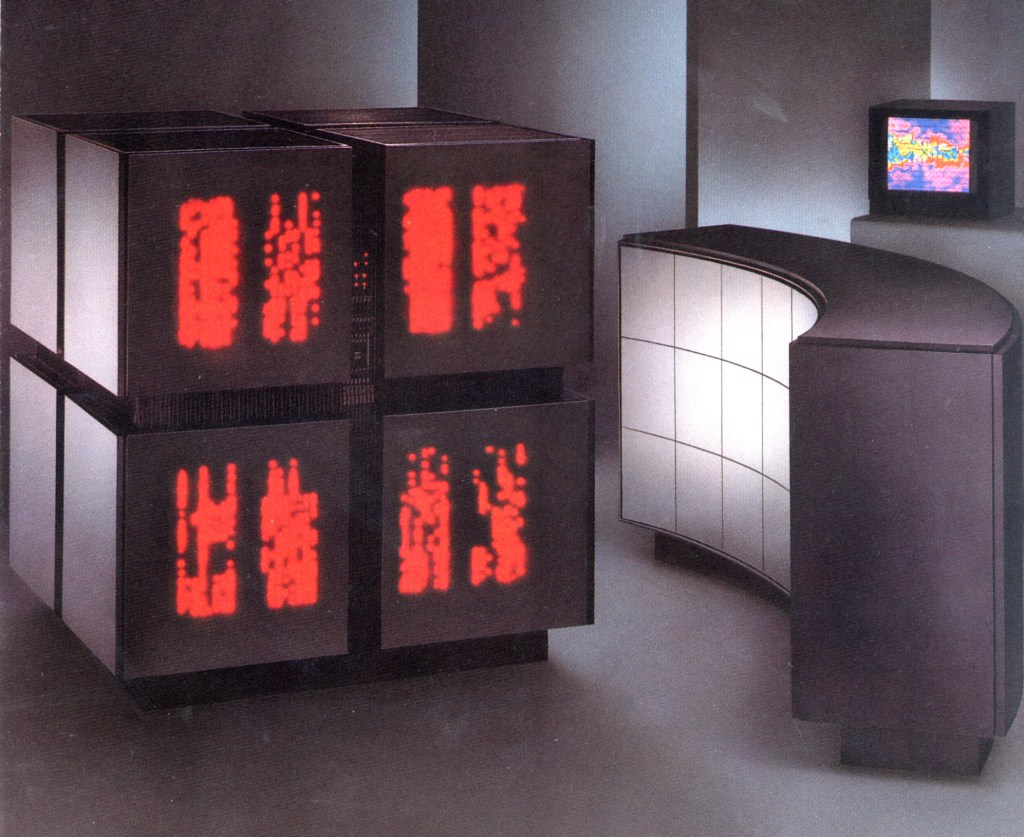
\includegraphics{images/tur-til-usa-1988/cm2.jpg}
	\caption{CM2 Connection Machine fra Thinking Machines Corp. inkludert det bardisk-formede disk-arrayet.}
\end{figure}

Dette firmaet påvirket til og med popkultur: det er blant annet flere henvisninger til dem og maskinene deres i Jurassic Park, som kom ut i 1993. På det tidspunktet var Connection Machine blant verdens raskeste datamaskiner; den inneholdt svært mange prosessorer (CM-1 og CM-2 hadde over 64 000 prosessorer), og hver av disse hadde direkte forbindelse til alle andre. En av de som var involvert i dette arbeidet var Richard Feynman, kjent fysiker og nobelprisvinner. Det er ikke trivielt å utnytte så mange prosessorer på en effektiv måte, og både hardware og software i Connection Machine var nøye designet for å maksimere effektivitet. Maskinene var også seriøst kule å se på, med et kubisk design med mengder av blinkene dioder og et array av harddisker som så mer ut som en bardisk enn noe annet. Bildet viser en CM-2 med 64 000 prosessorer og bardisk-formet disk-array. Firmaet gikk konkurs i 1994 og ble kjøpt av Sun Microsystems. 

\section{Besøk på AI-laben på MIT}

MITs Artificial Intelligence Laboratory var kjent for å være et sted hvor store ideer kom til verden, og det var blant annet der mye av det tidlige fundamentet for forskningen på kunstig intelligens (AI) ble lagt. Laben er også hjemmet til programmeringsspråket LISP, og var hvor Danny Hillis utviklet arkitekturen til Connection Machine, som, som tidligere omtalt, senere ble kommersialisert gjennom Thinking Machines Corporation. De fleste informatikere er nok også godt kjent med teksteditorene EMACS og GNUEMACS, som begge ble utviklet av Richard Stallman nettopp på MITs AI-lab. 

CYBs besøk på AI-laben fokuserte på deres robotforskning, og cybberne fikk se flere imponerende eksempler på roboter i aksjon under oppholdet. Etter demorunden, som inneholdt en informativ spørsmålsrunde, hørte vi et foredrag om AI-labens prosjekter. På forhånd hadde de blitt gjort oppmerksomme på at det var interesse for å få innsikt i deres tanker om framtiden til nevrale nettverk. Dette var et tema som på den tiden vakte stor interesse internasjonalt, og som det var høye forventninger til. Bakgrunnen til CYBs interesse for dette var at det var noe konkurranse mellom AI-miljøene og miljøene som jobbet med nevrale nettverk på den tiden. Det var likevel nokså uventet da Carl Hewitt, den ansvarlige for besøket på AI-laben, fortalte at han knapt syntes nevrale nettverk var verdt å jobbe med. Han mente det kanskje var rom for to-tre mastergradsprosjekter på temaet, men ikke mer. Marvin Minsky, som var en av grunnleggerne av laben, var også kjent for å ha et temmelig skeptisk syn på nevrale nettverk, og noen år senere døde interessen for nevrale nettverk nesten helt ut. Forventningene til feltet ble rett og slett ikke oppfylt. 

Noen få ildsjeler fortsatte imidlertid å studere dem, og for bare få år siden skjedde det et gjennombrudd i forskningen som ledet til det vi kaller Deep Learning. Deep Learning brukes i dag blant annet i Google Translate, i Apples Siri, til automatisk trading på New York børsen, og kan spille bedre poker enn profesjonelle pokerspillere. Om det er noe å lære av alt dette, så er det at det er vanskelig å spå langt fremover i tiden når det gjelder teknologisk utvikling. 

\section{Besøk på Computer Museum}

På den tiden var dette visstnok det eneste museet som i helhet var viet datafagets historie. Museet ga en lærerik og morsom innføring i både datamaskinens og programmeringens historie, og forsøkte seg også på noen fremtidsvisjoner. Det var mange hands-on demonstrasjoner, blant annet i bildebehandling, grafikk, bruk av roboter, kunstig intelligens og tale-gjenkjenning. I dag ville de fleste ha dratt kjensel på mange av disse anvendelsene fra sin egen mobiltelefon, men for 30 år siden var denne typen anvendelser langt fra dagliglivet og utrolig inspirerende å se og prøve. 

\section{Logistikk}

Flyet fra Boston til San Francisco skulle gå kl 06:10. Med tanke på distansen fra hotellet til flyplassen, og hvor tidlig på morgenen det var, ble det en utfordring å ordne transport, som Morten og Ole Christian ble gjort ansvarlige for. Løsningen deres var å dra ut til flyplassen selv og leie en bil, for så å hente resten i puljer. Det ble satt opp en plan der første avgang gikk fra hotellet 02:30, så 3:30, og så 4:30, med Ole Christian som sjåfør på alle turene. Noen må ha kommet seg dit på egenhånd, men klokken 5 var altså alle på flyplassen.

\section{San Francisco}

Turen gikk videre til San Francisco etter Boston, hvor det var planlagt to besøk: Amdahl og Sun. I San Fransisco ble det også en del nye opplevelser på de erkenorske cybberne, blant annet et første møte med jalapeño på en meksikansk restaurant, og mye spennende sightseeing. 

\section{Amdahl Corporation og Sun Microsystems}

Generelt var mottagelsen som sagt god hos alle de firmaene CYB besøkte, men Amdahl overgikk de andre med god margin. De hadde booket et konferanserom på et førsteklasses hotell, og stilte med så mange sjefer og så mye mat at man skulle tro de forventet ledelsen fra UiO, og ikke en gjeng studenter.

\begin{figure}
	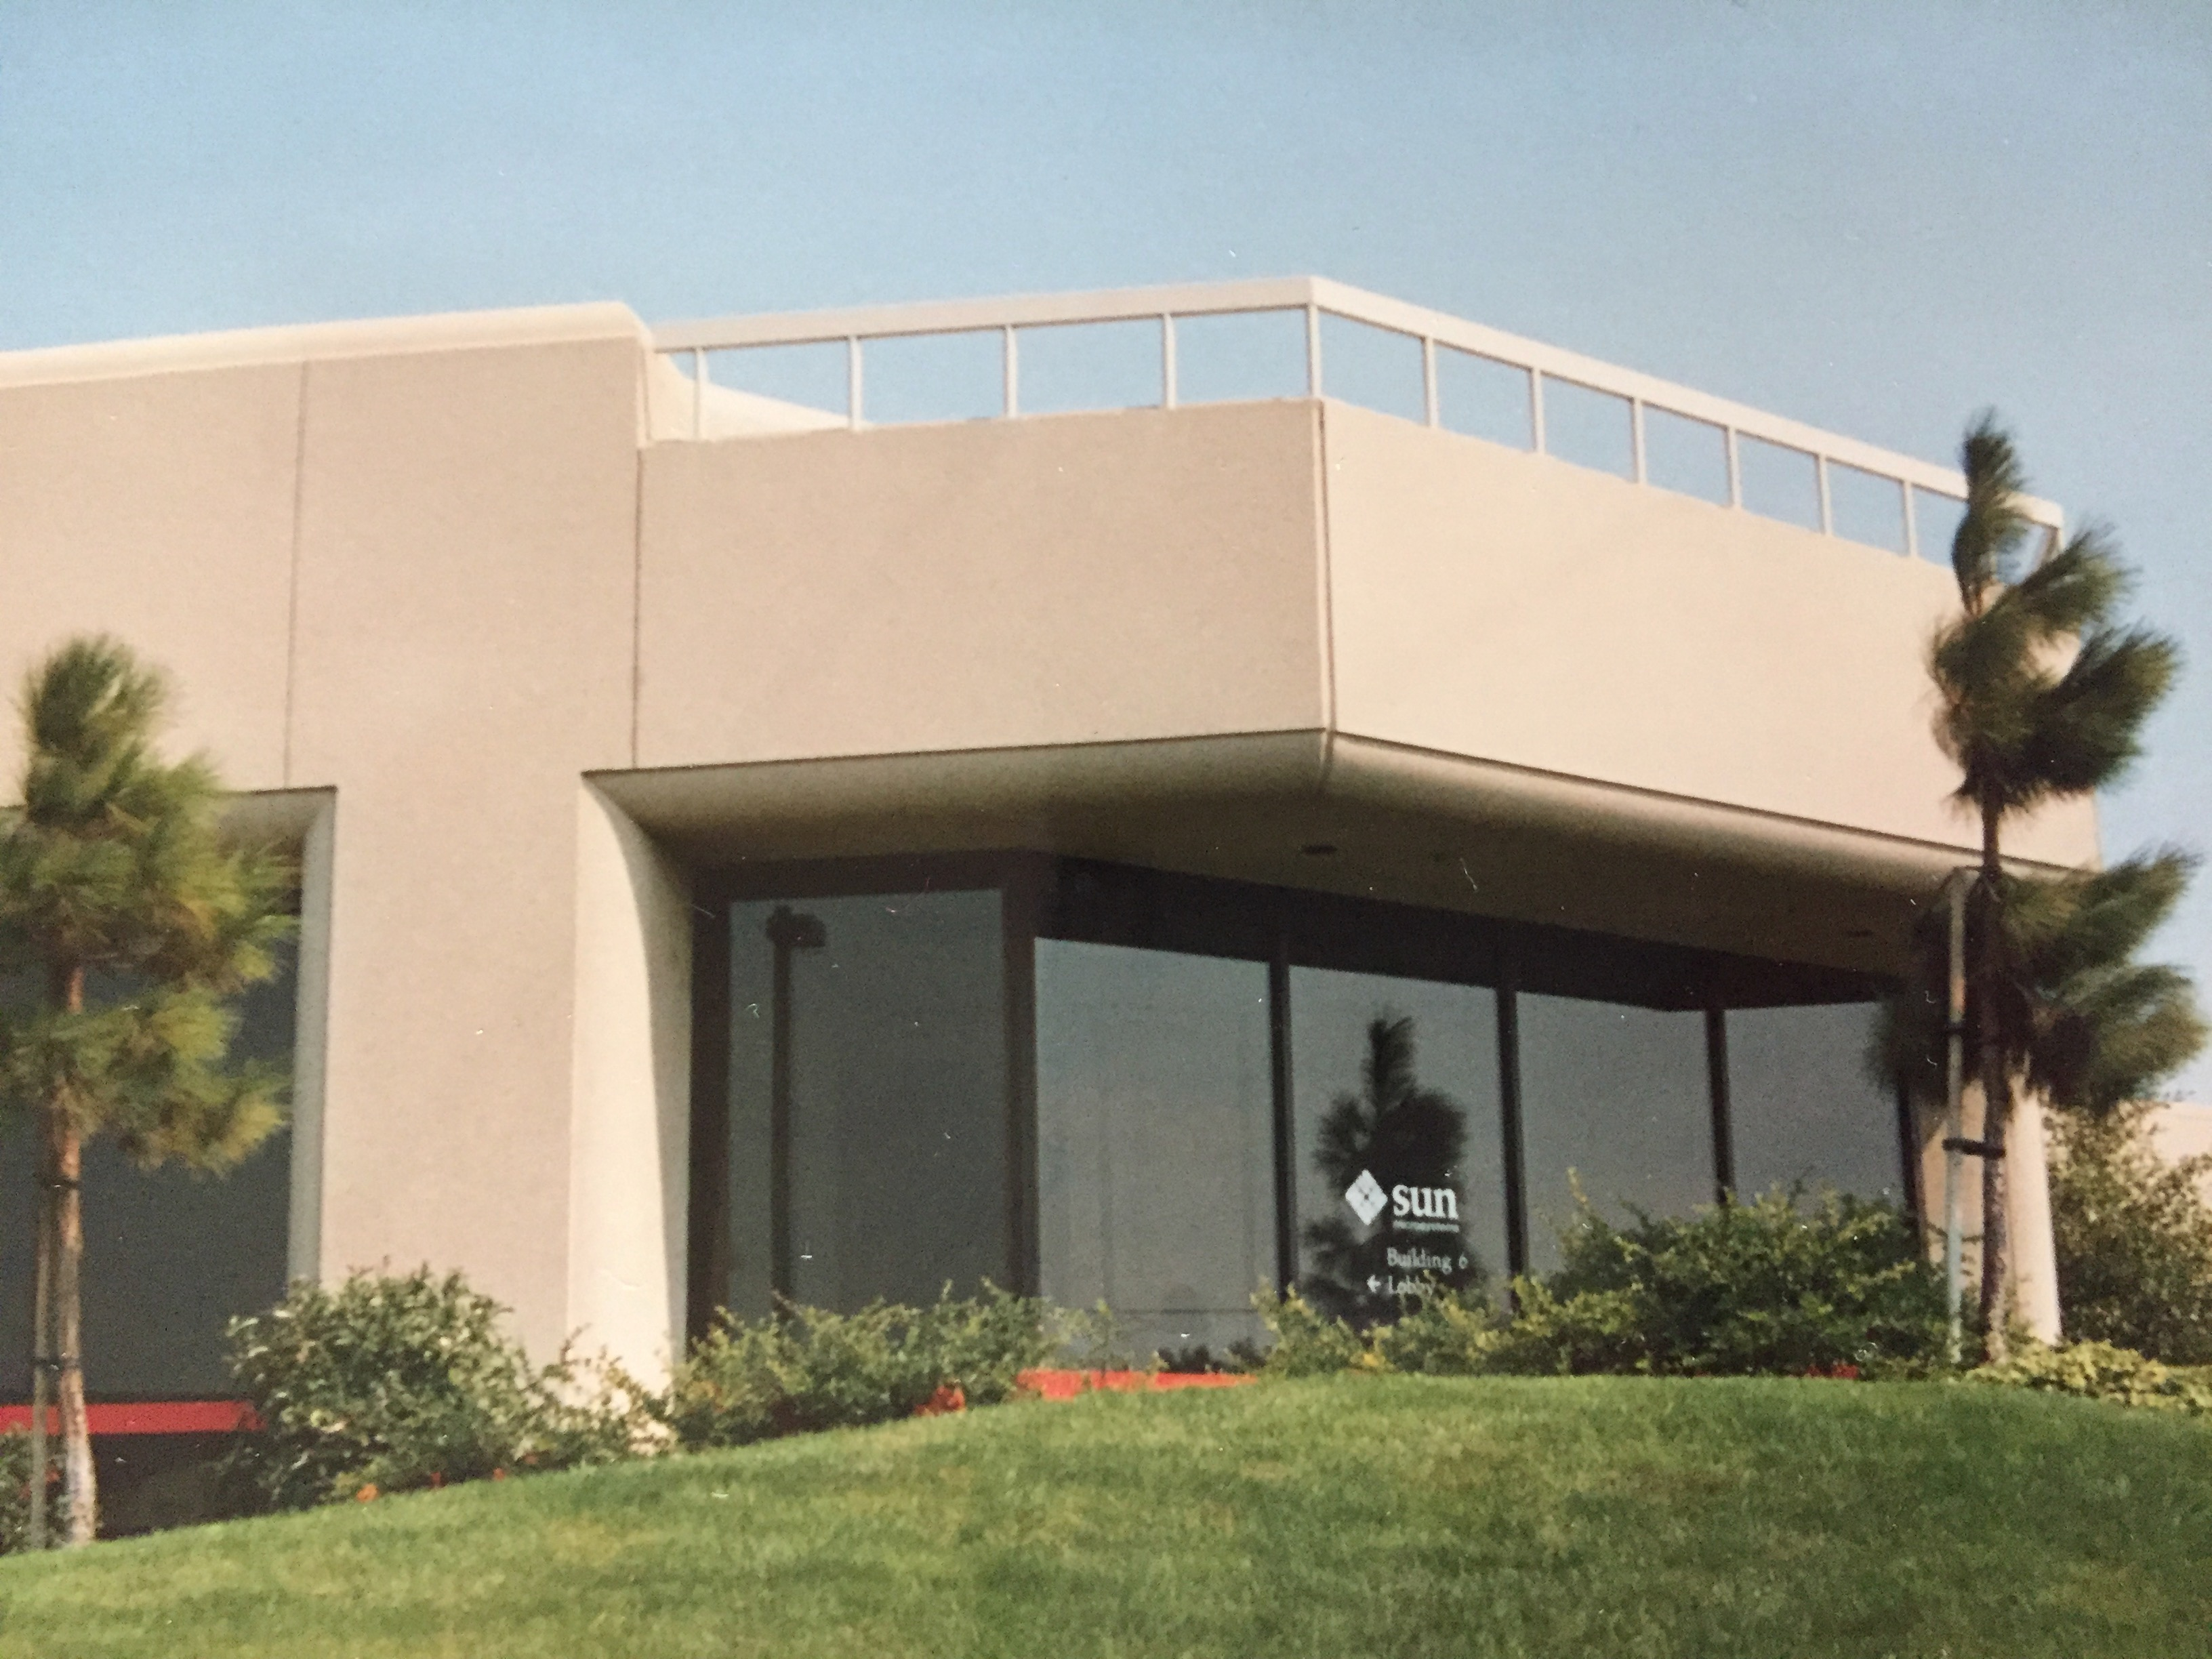
\includegraphics[width=\linewidth]{images/tur-til-usa-1988/IMG_3847.jpg}
	\caption{Sun Microsystems, Silicon Valley.}
\end{figure}

Sun, som var destinasjonen etter Amdahl, ble startet i 1982 av Vinod Khosla, Andy Bechtolsheim og Scott McNealyog. De var alle studenter ved Stanford og hadde sit hovedkvarter i Santa Clara i Silicon Valley. De ble fort ledende innen grafiske arbeidsstasjoner og var sentrale for utviklingen av Unix. CYB ble godt mottatt hos også her. De hadde lagt opp til å vise frem arbeidet sitt med grafiske brukergrensesnitt, hvor arbeidsstasjonene deres lå langt fremme. Det som Sun nå kanskje er mest kjent for er derimot programmeringsspråket Java, som ble utviklet der.

\section{Avslutning}

Etter Amdahl og Sun var det faglige over, og fra San Francisco bestemte cybberne for å splitte seg opp i mindre grupper og kjøre ned til Los Angeles for å tilbringe noen dager der. Morten, Øystein, Hans Henrik og Geir kjørte Highway One langs kysten i en Lincoln Town Car, som var en bil de var rimelig stolte over. På vei ned overnattet de i Santa Barbara, hvor de slo seg sammen med en av de andre gruppene.

\begin{figure}
	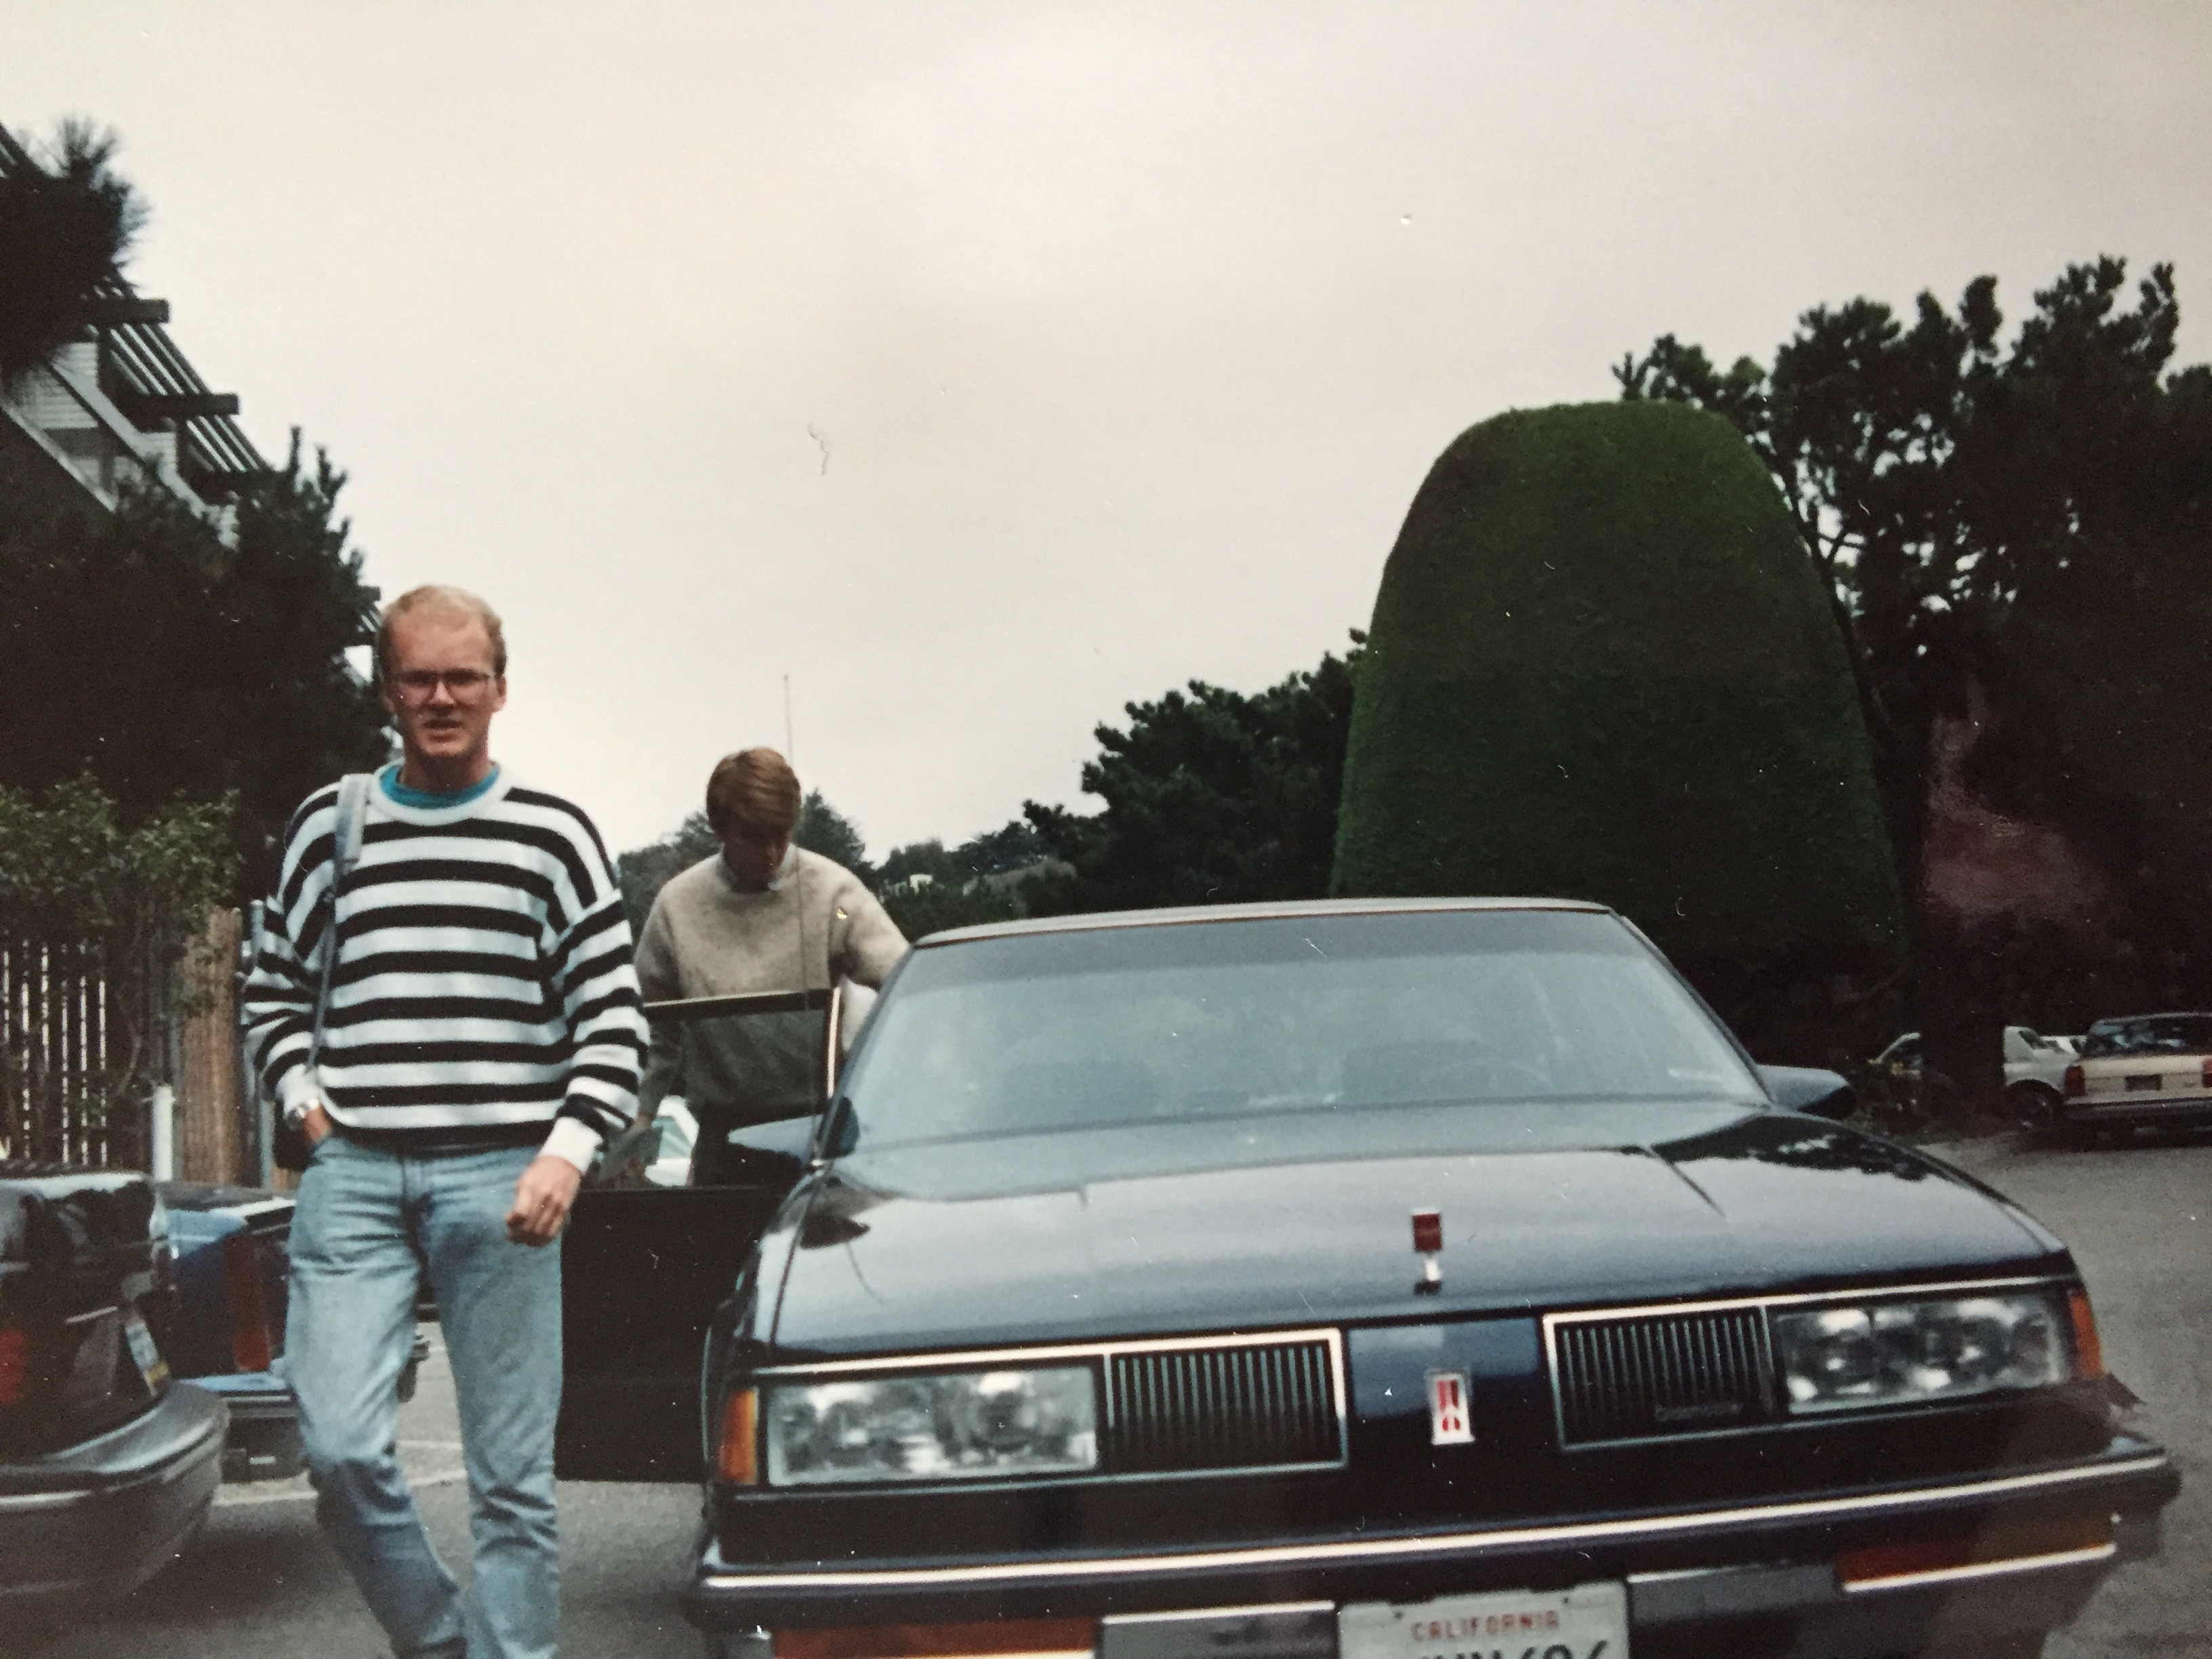
\includegraphics[width=\linewidth]{images/tur-til-usa-1988/IMG_3848.jpg}
	\caption{Stolte av leiebilen, en Lincoln Town Car, fra venstre: Geir Amdal, Hans Henrik Eriksen.}
\end{figure}

Etter noen dager i Los Angeles med sightseeing, Hollywood og Universal Studios gikk turen videre til Orlando, Florida, med fly. Her var det essensielt å få tatt turen innom Disney World og Epcot, samt utnytte muligheten for soling og bading. 

\begin{figure}[h!]
	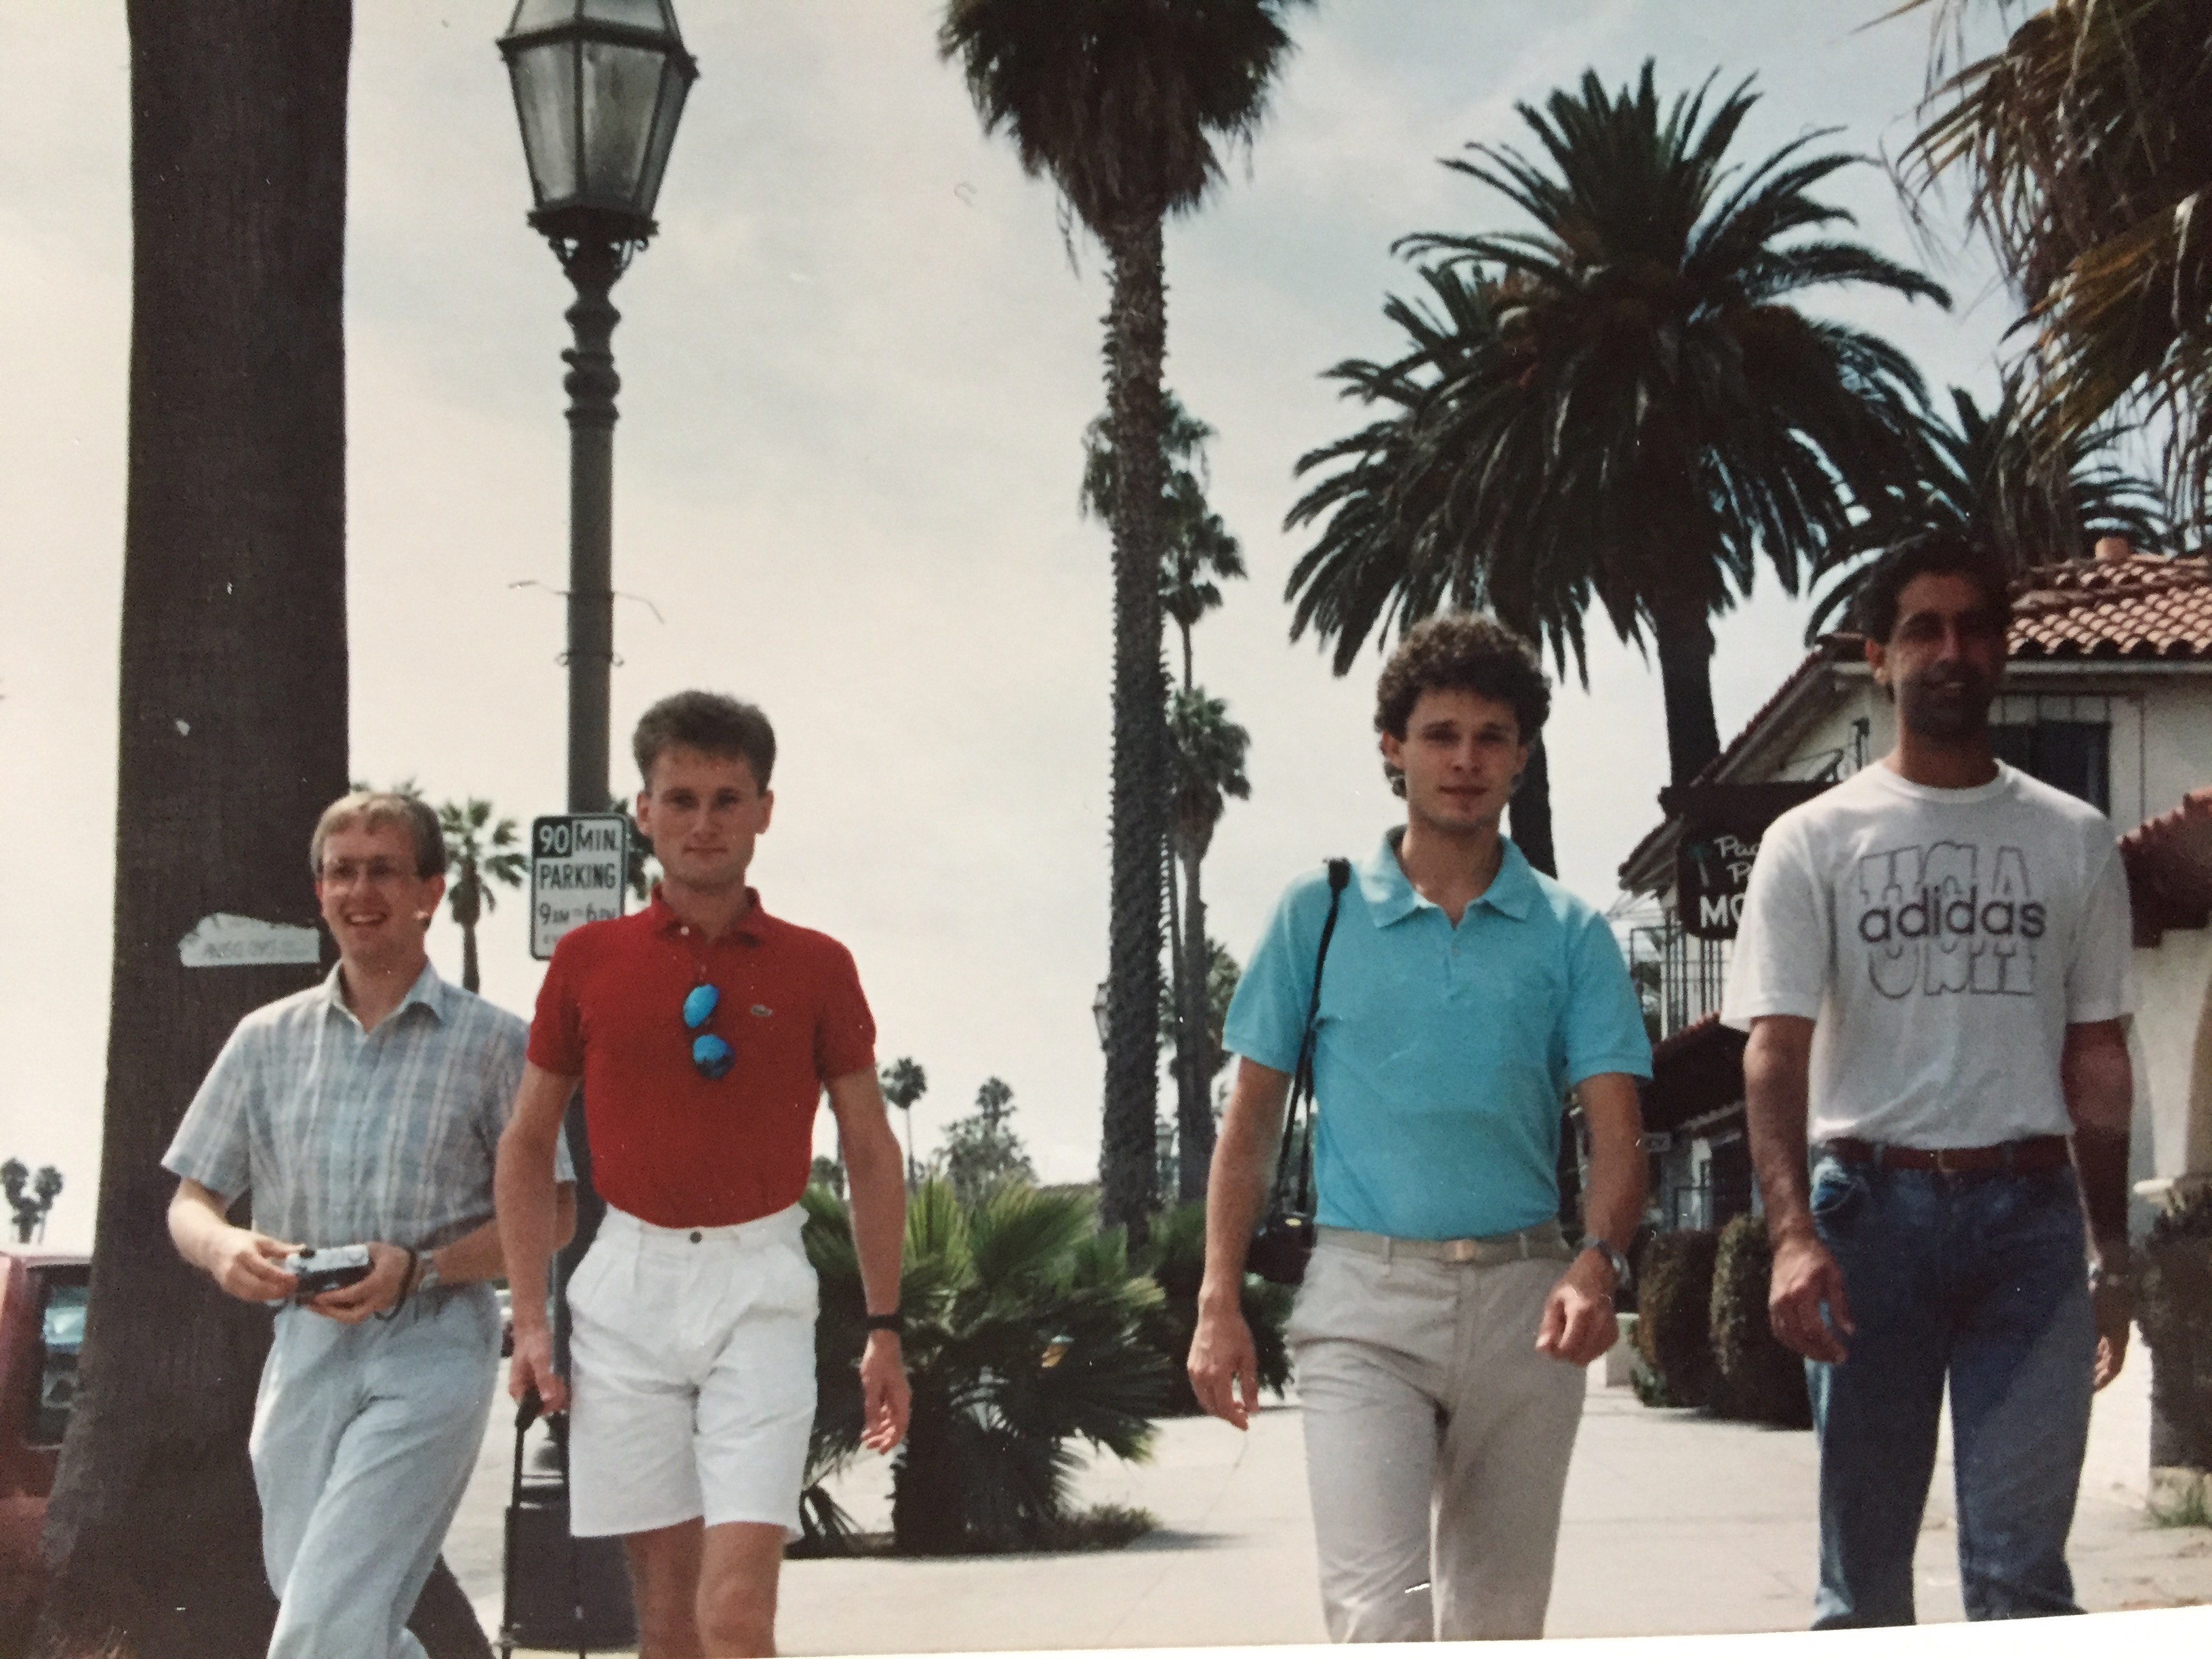
\includegraphics[width=\linewidth]{images/tur-til-usa-1988/IMG_3849.jpg}
	\caption{I Santa Barbara, fra venstre: Anders Ellefsrud, ukjent, Ole Christian Lingjærde, ukjent.}
\end{figure}

Noen fikk også tid til en tur til Kennedy Space Center. I 1988 var det en romferge som ble sendt opp, som tilfeldigvis skjedde akkurat i da CYB var i Orlando. Dette var den første romfergen som ble sendt opp etter den som eksploderte i 1986, og det var naturligvis mye oppmerksomhet rettet mot denne hendelsen. Det var blant annet mulig å kjøpe en mengde romfergerelaterte ting, som for eksempel frysetørket astronautis og The Space Shuttle Operators Manual. 

Da romfergen ble skutt opp var det noen cybbere i Disney World, blant annet Morten og Ole Christian, som fikk gleden av å være direkte vitner til romfergens ferd opp.

Denne turen står nok som et av høydepunktene i studietiden for de som var med: de fikk reist rundt i USA, opplevd mye og fikk besøkt noen av verdens største og mest innovative firmaer. Noe man kan tenke over i ettertid er at bortsett kanskje fra MIT, Apollo (som fortsatt kan ha noe arvegods i HP), og Sun (som det kan finnes spor av hos Oracle) er alle disse firmaene nå borte.
